\documentclass [t] {beamer} % KOMA script (article)

\mode<presentation> {
%\usetheme{boadilla}
%\usetheme{default}
%\usetheme{AnnArbor}
%\usetheme{Antibes}
%\usetheme{Bergen}
%\usetheme{Berkeley}
%\usetheme{Berlin}
%\usetheme{Boadilla}
%\usetheme{CambridgeUS}
%\usetheme{Copenhagen}
%\usetheme{Darmstadt}
%\usetheme{Dresden}
%\usetheme{Frankfurt}
%\usetheme{Goettingen}
%\usetheme{Hannover}
%\usetheme{Ilmenau}
%\usetheme{JuanLesPins}
%\usetheme{Luebeck}
\usetheme{Madrid}
%\usetheme{Malmoe}
%\usetheme{Marburg}
%\usetheme{Montpellier}
%\usetheme{PaloAlto}
%\usetheme{Pittsburgh}
%\usetheme{Rochester}
%\usetheme{Singapore}
%\usetheme{Szeged}
%\usetheme{Warsaw}

%\usecolortheme{albatross}
%\usecolortheme{beaver}
%\usecolortheme{beetle}
%\usecolortheme{crane}
%\usecolortheme{dolphin}
%\usecolortheme{dove}
%\usecolortheme{fly}
%\usecolortheme{lily}
%\usecolortheme{orchid}
\usecolortheme{rose}
%\usecolortheme{seagull}
%\usecolortheme{seahorse}
%\usecolortheme{whale}
%\usecolortheme{wolverine}

%\setbeamertemplate{footline} % To remove the footer line in all slides uncomment this line
%\setbeamertemplate{footline}[page number] % To replace the footer line in all slides with a simple slide count uncomment this line

%\setbeamertemplate{navigation symbols}{} % To remove the navigation symbols from the bottom of all slides uncomment this line
}

%\usepackage{beamerthemesplit}
\usepackage{appendixnumberbeamer}
%\usepackage{biblatex}
%\addbibresource{xampl.bib}

\usepackage{graphicx} % Allows including images
\usepackage{booktabs} % Allows the use of \toprule, \midrule and \bottomrule in tables
\usepackage{lipsum}
%\newcommand\fontup{\fontsize{20}{7.2}\selectfont}

\usepackage{amsmath}
%\interdisplaylinepenalty=2500
\usepackage{array}
%\hyphenation{op-tical net-works semi-conduc-tor}


\newcommand{\symb}[1]{\mbox{\boldmath${#1}$}}
\newcommand{\Ba}{\mbox{\boldmath$a$}}
\newcommand{\Bb}{\mbox{\boldmath$b$}}
\newcommand{\Bh}{\mbox{\boldmath$h$}}
\newcommand{\Bd}{\mbox{\boldmath$d$}}
\newcommand{\Be}{\mbox{\boldmath$e$}}
\newcommand{\Bg}{\mbox{\boldmath$g$}}
\newcommand{\Bf}{\mbox{\boldmath$f$}}
\newcommand{\Bi}{\mbox{\boldmath$i$}}
\newcommand{\Bj}{\mbox{\boldmath$j$}}
\newcommand{\Bp}{\mbox{\boldmath$p$}}
\newcommand{\Bq}{\mbox{\boldmath$q$}}
\newcommand{\Br}{\mbox{\boldmath$r$}}
\newcommand{\Bs}{\mbox{\boldmath$s$}}
\newcommand{\Bu}{\mbox{\boldmath$u$}}
\newcommand{\Bv}{\mbox{\boldmath$v$}}
\newcommand{\Bz}{\mbox{\boldmath$z$}}
\newcommand{\Bx}{\mbox{\boldmath$x$}}
\newcommand{\By}{\mbox{\boldmath$y$}}
\newcommand{\Beps}{\symb{\varepsilon}}
\newcommand{\BA}{\mbox{\boldmath$A$}}
\newcommand{\BC}{\mbox{\boldmath$C$}}
\newcommand{\BB}{\mbox{\boldmath$B$}}
\newcommand{\BD}{\mbox{\boldmath$D$}}
\newcommand{\BF}{\mbox{\boldmath$F$}}
\newcommand{\BG}{\mbox{\boldmath{$G$}}}
\newcommand{\BGA}{\mbox{\boldmath{$\Gamma$}}}
\newcommand{\BLA}{\mbox{\boldmath{$\Lambda$}}}
\newcommand{\BH}{\mbox{\boldmath$H$}}
\newcommand{\BU}{\mbox{\boldmath$U$}}
\newcommand{\BV}{\mbox{\boldmath$V$}}
\newcommand{\BO}{\mbox{\boldmath{$0$}}}
\newcommand{\BW}{\mbox{\boldmath$W$}}
\newcommand{\BI}{\mbox{\boldmath$I$}}
\newcommand{\BX}{\mbox{\boldmath$X$}}
\newcommand{\BP}{\mbox{\boldmath$P$}}
\newcommand{\BQ}{\mbox{\boldmath$Q$}}
\newcommand {\Min} {\mathop{\mbox{minimize}}}
\newcommand {\Max} {\mathop{\mbox{maximize }}}
\newcounter{abc}
\renewcommand{\theequation}{\arabic{equation}\alph{abc}}
\newcommand{\ome}{(\omega_1, \omega_2)}

\setbeamercolor{bibliography entry author}{fg=black}
 
%----------------------------------------------------------------------------------------
%	TITLE PAGE
%----------------------------------------------------------------------------------------

\title[Localization in PSN]{Localization Algorithms in Passive Sensor Networks} 

\author{Darya Ismailova} 
\institute[UVic] 
{
Department of Electrical and Computer Engineering \\
University of Victoria, Victoria, BC, Canada \\
\medskip
%\textit{ismailds@uvic.ca, wslu@uvic.ca} % Your email address
}
\date{January 19, 2017}

\begin{document} 
%\fontsize{14}{14}\selectfont

\begin{frame} % Slide 1
\titlepage 
\end{frame}


%----------------------------------------------------------------------------------------
%	PRESENTATION SLIDES
%----------------------------------------------------------------------------------------

%------------------------------------------------

\section{Introduction} 

\begin{frame} % Slide 2
\frametitle{Outline} 
\begin{enumerate}
\item
Motivation
\\~\\
\item
Basic Localization Systems and Methods
\\~\\
\item
Iterative Re-Weighting Least-Squares Methods for Source Localization
\\~\\
\item
Penalty Convex-Concave Procedure for Range-based Localization
\\~\\
\item
Conclusions and Future Work
\end{enumerate}
\end{frame}


\begin{frame} % Slide 3
\frametitle{Introduction}
\phantom{m}
\begin{itemize}
\item
Navigation: outdoor; indoor
\\~\\
\item
Surveillance
\\~\\
\item
Localization of emergency callers
\\~\\
\item
Emergency and rescue operations / first responders
\\~\\
\item
Self-organizing networks
\\~\\
\item
Asset monitoring and tracking
\\~\\
\item
Other commercial location-based services
\\~\\
\item
\ldots
\end{itemize}
\end{frame}

\begin{frame} % Slide 4
\frametitle{Introduction}
\phantom{m}
\begin{itemize}
\item
Ranging methods
\begin{itemize}
\item
range measurements (Time Of Arrival)
\item
range-difference measurements (Time-Difference of Arrival)
\item
received signal strength
\\~\\
\end{itemize}

\item
Angle Of Arrival Techniques
\\~\\
\item
Survey-Based Systems (fingerprinting)
\begin{itemize}
\item
memoryless systems (SVM, NN)
\item
memory systems (Bayesian inference, grid-based Markov)
\item
channel impulse response fingerprinting
non-RF features
\end{itemize}
\end{itemize}
\end{frame}

\begin{frame} % Slide 5
\frametitle{Basic Localization Systems and Methods}
\begin{figure}[h]
%\centering
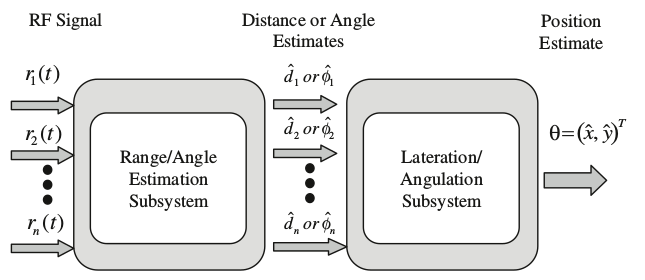
\includegraphics[width=1.0\textwidth]{../figures/localization_example.png}
\caption{Classical geolocation system. Range or angle information is extracted from received RF signals. Location is then estimated by lateration/angulation techniques [GeoLoc].}
\label{fig:2step}
\end{figure}
\end{frame}

\begin{frame} % Slide 6
\frametitle{Time Of Arrival Localization (TOA)}
\begin{figure}[h]
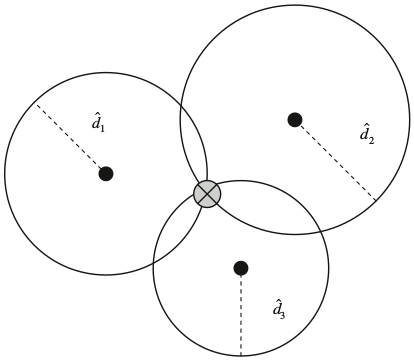
\includegraphics[height=0.6\textheight]{../figures/toa_example.png}
\caption{TOA-based trilateration. Range measurements to at least three BS make
up a set of nonlinear equations that can be solved to estimate the position of a
signal source [GeoLoc].}
\label{fig:2step}
\end{figure}
\end{frame}

\begin{frame} % Slide 7
\frametitle{Time Of Arrival Localization (TOA)}
\phantom{m}
The nonlinear least squares (NLLS) source location extimate $\hat{\Bx}$ is found by
\begin{equation}
\nonumber
\hat{\Bx} = \mbox{argmin}_{\Bx}\left\lbrace \sum_{i=1}^m \beta_i\left(d_n^i - \|\Bx -  \Ba_i \| \right)^2 \right\rbrace
\end{equation}
where 
\\
$\Ba_i$- a vector of known coordinates of reference points (sensors)
\\~\\
$d_n^i $ - a noisy range measurement associated with it
\\~\\
$\beta_i$ - a weight used to emphasize the degree of confidence in the
measurement
\\~\\
$m$ - the number of sensors.
\end{frame}

\begin{frame} % Slide 8
\frametitle{Time-Difference Of Arrival Localization (TDOA)}
\begin{figure}[h]
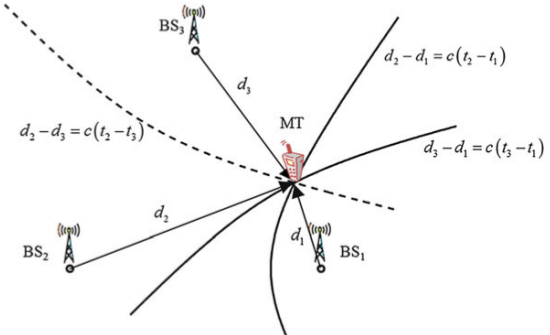
\includegraphics[height=0.7\textheight]{../figures/tdoa_example.png}
\caption{Example of observed time-difference of arrival (O-TDOA) method [GeoLoc].}
\label{fig:2step}
\end{figure}
\end{frame}

\begin{frame} % Slide 9
\frametitle{Time-Difference Of Arrival Localization (TDOA)}
\phantom{m}
Given the range-difference measurements
\begin{equation}
\nonumber
d_i = \|\Bx -  \Ba_i \| - \|\Bx -  \Ba_0 \| = \|\Bx -  \Ba_i \| - \|\Bx\|, \mbox{for } i = 1, 2, \ldots, m
\end{equation}
The standard NLLS location estimate $\hat{\Bx}$ is found by
\begin{equation}
\nonumber
\hat{\Bx} = \Min_{\Bx} \sum_{i=1}^m \left(\|\Bx -  \Ba_i \| - \|\Bx\| - d_n^i\right)^2
\end{equation}
with 
\\
$\Ba_i$- a vector of known coordinates of reference points (sensors)
\\
$d_n^i $ - a noisy range-difference measurement associated with it
\\
$m$ - the number of sensors.
\end{frame}



\begin{frame} % Slide 10
\frametitle{Methods Based on Received Signal Strength (RSS-based)}
\phantom{m}
The relationship between the RSS reading and the distance can be
approximated by
\begin{equation}
\nonumber
P_x(d) = P_0(d_0) - 10n_p\log_{10}\left( \frac{d_i}{d_0}\right) + X_{\sigma}
\end{equation}
where
\\
$P_0(d_0)$ - a reference power in dB milliwatts at a reference distance $d_0$ away from the transmitter
\\
$n_p$ - the pathloss exponent
\\
$X_{\sigma}$ - the log-normal shadow fading component with variance $\sigma^2$
\\
$d_i$ - the distance between the mobile devices and the ith base station
\\
$\sigma$ and $n_p$ are environment dependent
\end{frame}


\begin{frame} % Slide 11
\frametitle{Why Least Squares}
\phantom{m}
\begin{itemize}
\item
Least squares (LS) algorithms for range-based localization:\\
- geometrically meaningful\\
- provide low complexity solutions with competitive accuracy
\\~\\
\item
However:\\
- the error measure is non-convex\\
- excludes many local methods, that are iterative
\\~\\
\item
Solutions obtained using global localization techniques such as
semidefinite programming (SDP) are not optimal in LS sense.
\end{itemize}
\end{frame}


\begin{frame} % Slide 12
\frametitle{Iterative Re-Weighting Least-Squares Methods for Source
Localization}
\phantom{m}
\begin{itemize}
\item
Methods developed by A. Beck, P. Stoica, J. Li [BSL2008] for \textit{squared} range LS (SR-LS) and \textit{squared} range difference LS (SDR-LS) problems allow to obtain exact and \textit{global}  solutions.
\\~\\
\item
The results produced are merely approximations of the original LS
problems because SR-LS and SRD-LS are no longer an ML solutions.
\\~\\
\item
Proposed iterative procedure where the SR-LS (or SRD-LS) algorithm is applied to a \textit{weighted} sum of squared terms and special weights construction allow to obtain a solution which is considerably closer to
the original range-based (or range-difference-based) LS solution.
\end{itemize}
\end{frame}




\section[Chapter 2]{Iterative Re-Weighting Least-Squares Methods for Source Localization}

\subsection{Range-Based Localization} %2.2

\begin{frame} % Slide 13
\frametitle{Source Localization From Range Measurements}
{\large \textit{Measurement Model}} \\~\\
\normalsize
\begin{itemize}
\item 
Throughout it is assumed that \textit{range measurements} obey the model
\begin{equation} 
\nonumber
%\setcounter{equation}{1}
r_i = \|{\Bx} - {\Ba}_i\| + \varepsilon_i, \quad i = 1, \ldots , m.
\end{equation}  
where $\{\Ba_1,\ldots, \Ba_m\}$ - given array of $m$ sensors;\\
$\Ba_i\in R^n$  contains $n$ coordinates of the $i$th sensor in space $R^n$; \\
$r_i$ - received noisy distance reading from the $i$th sensor; \\
$\varepsilon_i$ - unknown noise associated with measurement from the $i$th sensor. 
\\~\\
\item
The problem can be stated as to estimate the exact source location $\Bx \in R^n$ from noisy range measurements $\Br = [r_1 \ r_2 \ldots r_m]^T$.
\end{itemize}
\end{frame}



\begin{frame} % Slide 14
\frametitle{Source Localization From Range Measurements}
{\large \textit{LS Formulations}} \\~\\
\normalsize
\begin{itemize}
\item 
The range-based least squares (R-LS) estimate refers to the solution of the problem
\begin{equation} \label{R} 
\Min_{\Bx} f(\Bx)=\sum_{i=1}^{m} (r_i - \|{\Bx} - {\Ba}_i\|)^2	\tag{R}
\end{equation} \\
\item If $\Beps \sim N(0,\symb{\Sigma}) $ and $\symb{\Sigma} \propto \BI$, then the R-LS solution of problem \eqref{R} is identical to the ML location estimator. \\ ~\\
%This formulation is connected to the ML estimator that determines source location by examining the probabilistic model of  $\Beps$. \\~\\
 \item  Unfortunately, the objective in \eqref{R} is highly non-convex, possessing many local minimizers even for small-scale systems.
\end{itemize}
\end{frame}



\begin{frame}
\frametitle{Source Localization From Range Measurements}
{\large \textit{LS Formulations}} \\~\\
\normalsize
\begin{itemize}
\item 
Alternatively, location estimate can be obtained by solving the \textit{squared range based LS} (SR-LS) problem [BSL2008]
\begin{equation} \label{SR}
\Min_{\Bx} \sum_{i=1}^{m} (\|{\Bx} - {\Ba}_i\|^2 - r_i^2)^2 \tag{SR}
\end{equation}

\item  
The SR-LS estimate is no longer an ML solution, hence, only an approximation of the original R-LS problem.\\
\item 
To reduce the gap between the two solutions we propose a weighted SR-LS (WSR-LS) problem:
\begin{equation} \label{WSR}
\Min_{\Bx} \sum_{i=1}^{m} w_i\left(\|{\Bx} - {\Ba}_i\|^2 - r_i^2\right)^2 \tag{WSR}
\end{equation}
\end{itemize}
\end{frame}



\begin{frame} % Slide 16
\frametitle{Source Localization From Range Measurements}
{\large \textit{An Iterative Re-Weighting Strategy}} \\~\\
\normalsize
\begin{itemize}
\item 
WSR-LS with properly chosen weights facilitates an excellent approximation of the R-LS estimate. \\~\\

\item 
The main idea is to use the weights ${w_i, i = 1, \ldots, m}$ to tune the objective in \eqref{WSR} toward the objective in \eqref{R}. % \\~\\
%\item
%To substantiate the idea, 
%To see this we 
%We compare the $i$th term of the objective in \eqref{WSR} with its counterpart in \eqref{R} as:
\begin{equation} 
\nonumber
\underbrace{w_i\left(\|\Bx-\Ba_i\|^2-r_i^2\right)^2}_{\mbox{in (WSR)}}\leftrightarrow\underbrace{\left(\|\Bx-\Ba_i\|-r_i\right)^2}_{\mbox{in (R)}}
\end{equation}
\end{itemize}
\end{frame}



\begin{frame} % Slide 17
\frametitle{Source Localization From Range Measurements}
{\large \textit{An Iterative Re-Weighting Strategy}} \\~\\
\normalsize
\begin{itemize}
\item 
By writing the $i$th term in \eqref{WSR} as
\begin{equation}
\nonumber
\begin{array}{l}
w_i\left(\|\Bx-\Ba_i\|^2-r_i^2\right)^2 = w_i\left(\|\Bx-\Ba_i\|+r_i\right)^2 \underbrace{\left(\|\Bx-\Ba_i\|-r_i\right)^2}_{\mbox{same as in (R)}}
\end{array}
\end{equation}
we note that the objective in \eqref{WSR} would be the same as in \eqref{R} if the weight $w_i$ was assigned to $1/\left(\|\Bx-\Ba_i\|+r_i\right)^2$. \\~\\
\item 
Evidently, such weight assignments cannot be realized.
\end{itemize}
\end{frame}


\begin{frame}% Slide 17
\frametitle{Source Localization From Range Measurements}
{\large \textit{An Iterative Re-Weighting Strategy}} 
\\~\\
\normalsize

\begin{itemize}
\item 
 In the proposed iterative procedure we solve a weighted SR-LS sub-problem,where at each iteration the weights are fixed:
\begin{equation} \label{IRWSR}
\Min_{x} \sum_{i=1}^m w_i^{(k)}\left(\|\Bx-\Ba_i\|^2-r_i^2\right)^2 \tag{IRWSR}
\end{equation}
\item 
 for $k=1$ all weights $\{w_i^{(1)}, i=1,\ldots, m\}$ are set to unity; \\
 \item 
 for $k\geq2$ the weights $\{w_i^{(k)},i=1,\ldots,m\}$ are assigned using the previous iterate $\Bx_{k-1}$ as
\begin{equation} 
\nonumber
w_i^{(k)}=\frac{1}{\left(\|\Bx_{k-1}-\Ba_i\|+r_i\right)^2}.
\end{equation}

\end{itemize}
\end{frame}



%\section[SRD-LS Methods]{Source Localization From Range-Difference Measurements}
\subsection{Range-Difference-Based Localization} %2.2

%------------------------------------------------

\begin{frame} % Slide 19
\frametitle{Source Localization From Range-Difference Measurements} %3.2
{\large \textit{Problem Statement}}
\\~\\
\normalsize
\begin{itemize}
\item 
It is assumed that the range-difference measurements obey the model:
 \begin{equation} 
 \nonumber
 d_i=\|\Bx-\Ba_i\|-\|\Bx-\Ba_0\|=\|\Bx-\Ba_i\|-\|\Bx\|, \quad i = 1,\ldots,m
 \end{equation}
where $\Ba_0$ - reference sensor placed at the origin.\\~\\
 \item 
 The standard range-difference LS (RD-LS) problem is formulated as
 \begin{equation} \label{RD}
\Min_{\Bx \in R^n} F(\Bx)=\sum_{i=1}^m \left(d_i+\|\Bx\|-\|\Bx-\Ba_i\|\right)^2 \tag{RD}
 \end{equation}
 \end{itemize}
\end{frame}



\begin{frame} % Slide 20
\frametitle{Source Localization From Range-Difference Measurements} %3.2
{\large \textit{SRD-LS and WSRD-LS formulations}}
\\~\\
\normalsize
\begin{itemize}
\item 
An approximation of the RD-LS solution can be obtained by solving the \textit{squared range difference based LS} (SRD-LS) problem. \\ % [BSL2008]. \\
\item 
By re-writing the measurements model as $d_i+\|\Bx\|=\|\Bx-\Ba_i\|$ and squaring both sides, we obtain
  \begin{equation} 
  \nonumber
-2d_i\|\Bx\|-2\Ba_i^T\Bx=g_i, \quad i=1,\ldots,m
 \end{equation}
 where $g_i=d_i^2-\|\Ba_i\|^2$.  
The SRD-LS solution can be obtained by minimizing following criterion:
 \begin{equation}
 \nonumber
\Min_{{\Bx} \in R^{n}} \sum_{i=1}^m \left(-2\Ba_i^T\Bx-2d_i\|\Bx\|-g_i\right)^2 
\end{equation}

 \end{itemize}
\end{frame}


\begin{frame} % Slide 21
\frametitle{Source Localization From Range-Difference Measurements} 
{\large \textit{Improved Solution Using Iterative Re-weighting}} \\~\\
\normalsize
\begin{itemize}
\item 
We now present a method for improved solutions over SRD-LS solutions. 
\\~\\
\item 
We consider the weighted SRD-LS problem
\begin{equation} \label{WSRD}
\Min_{{\Bx} \in R^n} \sum_{i=1}^m w_i\left(-2\Ba_i^T\Bx-2d_i\|\Bx\|-g_i\right)^2 \tag{WSRD}
\end{equation}
where weights $w_i$ for $i=1,\ldots,m$ are \textit{fixed} nonnegative constants. 
\end{itemize}
\end{frame}



\begin{frame} % Slide 22
\frametitle{Source Localization From Range-Difference Measurements} %3.2
{\large \textit{Improved Solution Using Iterative Re-weighting}} 
\\~\\
\normalsize
\begin{itemize}
\item <1->
The $i$th term of the objective function in \eqref{WSRD} can be written as:
\begin{equation}
\nonumber
\begin{aligned}
&w_i\left(-2d_i\|\Bx\|-2\Ba_i^T\Bx-g_i\right)^2 \\
%= &w_i\left((d_i+\|\Bx\|)^2-\|\Bx-\Ba_i\|^2\right)^2 \\
=&w_i\left(d_i+\|\Bx\|+\|\Bx-\Ba_i\|\right)\underbrace{\left(d_i+\|\Bx\|-\|\Bx-\Ba_i\|\right)}_{\mbox{same as in RD}}
\end{aligned}
\end{equation}
\\

\phantom{m} 
\item 
If weights $w_i$ were set to $1/\left(d_i+\|\Bx\|+\|\Bx-\Ba_i\|\right)^2$  the objective in \eqref{WSRD} would be the same as in \eqref{RD}. 
\end{itemize}
\end{frame}



\begin{frame} % Slide 23
\frametitle{Source Localization From Range-Difference Measurements} %3.2
{\large \textit{Improved Solution Using Iterative Re-weighting}} 
\\~\\
\normalsize
\begin{itemize}
\item 
We employ an iterative procedure  where the weights in the $k$th iteration are assigned to 
\begin{equation} 
\nonumber
w_i^{(k)}=\frac{1}{\left(d_i+\|\Bx_{k-1}\|+\|\Bx_{k-1}-\Ba_i\|\right)^2}, i=1,\ldots,m
\end{equation} \\~\\
with $\{w_i^{(1)} = 1, i=1,\ldots, m\}$.
 \\~\\
\item 
We will refer to the derived problem as the iterative re-weighted SRD-LS (WSRD-LS) problem and the solution obtained as IRWSRD-LS solution. 

\end{itemize}
\end{frame}


\subsection{Numerical Results}
\begin{frame} % Slide 24

\frametitle{Performance Evaluation for SR-LS and IRWSR-LS} 
\normalsize
\begin{itemize}
\item 
We can see that IRWSR-LS solutions offer considerable improvement over SR-LS solutions.
\begin{table}
\caption[c]{Averaged MSE for SR-LS and IRWSR-LS methods by noise level}
\begin{tabular}{|c|c|c|c|}
\toprule
\textbf{$\sigma$ } & \textbf{SR - LS} & \textbf{IRWSR-LS } & \textbf{Improvement (\%)}\\
\midrule 
1e-03&	2.03251062e-06&	1.19962894e-06& 41	\\ &&&\\
1e-02&	1.83717590e-04&	1.24797437e-04& 32	\\ &&&\\
1e-01&	1.83611315e-02&	1.22233840e-02& 33	\\ 
\bottomrule
\end{tabular}
\end{table}

\end{itemize}
\end{frame}


\begin{frame} % Slide 25
%\frametitle{An Iterative Re-Weighting Strategy}
\frametitle{Performance Evaluation for SRD-LS and IRWSRD-LS} 
\normalsize

\begin{table}
\caption{Averaged MSE for SRD-LS and IRWSRD-LS methods by noise level}
\begin{tabular}{|c|c|c|c|}
\toprule
\textbf{$\sigma$ } & \textbf{SRD - LS} & \textbf{IRWSRD-LS } & \textbf{Improvement (\%)}\\
\midrule
1e-04&	1.38301598e-08&	8.22705918e-09& 40\\ &&&\\
1e-03&	1.60398717e-06&	1.03880406e-06& 35\\ &&&\\
1e-02&	1.11632818e-04&	6.67785604e-05& 40\\ &&&\\
1e-01&	1.20947651e-02&	7.20891487e-03& 40\\ &&&\\
1e+0&	1.57050323e+00&	9.70756420e-01& 40\\ %&&&&\\
\bottomrule
\end{tabular}
\end{table}
\end{frame}

%\section{Penalty Convex-Concave Procedure for Source Localization}
\section[Chapter 3]{PCCP for Source Localization}


\begin{frame} % Slide 26
\frametitle{Problem Statement }
{\large \textit{Measurement Model}} \\~\\
\normalsize
\begin{itemize}
\item
The \textit{range measurements} model is assumed to be given by
\begin{equation} 
\nonumber
r_i = \|{\Bx} - {\Ba}_i\| + \varepsilon_i, \quad i = 1, \ldots , m.
\end{equation}  
$\{\Ba_1,\ldots, \Ba_m\}$ - given array of $m$ sensors;\\
$r_i$ - received noisy distance reading from sensor $i$; \\
$\varepsilon_i$ - unknown noise associated with measurement from the $i$th sensor. \\ ~\\

\item
The range-based least squares  estimate refers to the solution of% the problem
\begin{equation} \label{R-LS} 
\Min_{\Bx} F(\Bx)=\sum_{i=1}^{m} (r_i - \|{\Bx} - {\Ba}_i\|)^2	\tag{R}
\end{equation}
\end{itemize}
\end{frame}

\begin{frame} % Slide 27
\frametitle{}
\phantom{m}
\begin{itemize}
\item
We frame the localization problem as difference-of-convex-functions
(DC) program.
\\~\\
\item
Proposed formulation:\\
- based on a penalty convex-concave procedure (PCCP)\\
- accepts infeasible initial points\\
- additional constraints that enforce the algorithms iteration path
towards the LS solution\\
- strategies to secure good initial points
\end{itemize}
\end{frame}


\subsection{Fitting the Localization Problem to the CCP Framework}

\begin{frame} % Slide 28
\frametitle{Basic Convex-Concave Procedure (CCP)} 
\phantom{m}
\begin{itemize}
\item
The CCP finds local optima of \textit{nonconvex} problems of the  form
\begin{eqnarray} \label{eq:5}
 \Min_{\Bx} & {} & f(\Bx) - g(\Bx) \nonumber 
\\ \mbox{subject to:} & {} & f_i(\Bx) \leq g_i(\Bx) \quad \mbox{for: }  i = 1, 2, \ldots, m  \nonumber 
\end{eqnarray}
where $f(\Bx), g(\Bx) , f_i(\Bx), g_i(\Bx)$ for $i = 1, 2 \ldots, m$ are convex. 
\\~\\

\item 
It is a descent algorithm that requires a \textit{feasible} initial point $\Bx_0$, i.e. $f_i(\Bx) - g_i(\Bx) \leq 0$ for $i = 1, 2 \ldots, m$.
\end{itemize}
\end{frame}


\begin{frame}  % Slide 29
\frametitle{Basic Convex-Concave Procedure (CCP)} 
\phantom{m}
\begin{itemize}
\item
 The basic CCP algorithm is an iterative procedure including two key steps (in the $k$-th iteration): \\~\\% where iterate $\Bx_k$ is known): \\~\\
\begin{enumerate}
\item
Convexify: form $\hat{g}(\Bx,\Bx_k)  =   g(\Bx_k) +  \bigtriangledown g(\Bx_k)^T(\Bx - \Bx_k) $ \\~\\
 \qquad \qquad  \quad and $\hat{g}_i(\Bx,\Bx_k)  =   g_i(\Bx_k) +  \bigtriangledown g_i(\Bx_k)^T(\Bx - \Bx_k) $ \\
 \qquad \qquad \qquad for $ i = 1, 2 \ldots, m $
\\~\\
\item
Solve  the convex problem:
\linespread{0.1}\selectfont
\begin{eqnarray} 
 \Min_{\Bx} & &  f(\Bx) - \hat{g}(\Bx, \Bx_k) \nonumber
\\ \mbox{subject to:} & &  f_i(\Bx) -  \hat{g}_i(\Bx, \Bx_k) \leq 0   \nonumber
\\ \quad & & \mbox{for: }  i = 1, 2, \ldots, m \nonumber
\end{eqnarray} \\~\\
\linespread{1}\selectfont
\end{enumerate}

\end{itemize}
\end{frame}

\begin{frame} % Slide 30
\frametitle{An example of the basic CCP procedure}
\begin{figure}[h]
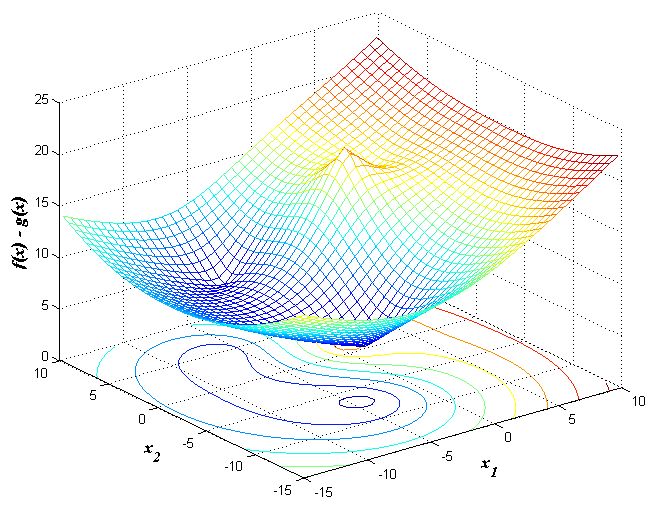
\includegraphics[height=0.7\textheight]{../figures/ccp/ccp_a.png}
\caption{A nonconvex function in the form of the difference of two convex
functions and its contour plot.}
\label{fig:ccp_a}
\end{figure}
\end{frame}

\begin{frame} % Slide 31
\frametitle{An example of the basic CCP procedure}
\begin{figure}[h]
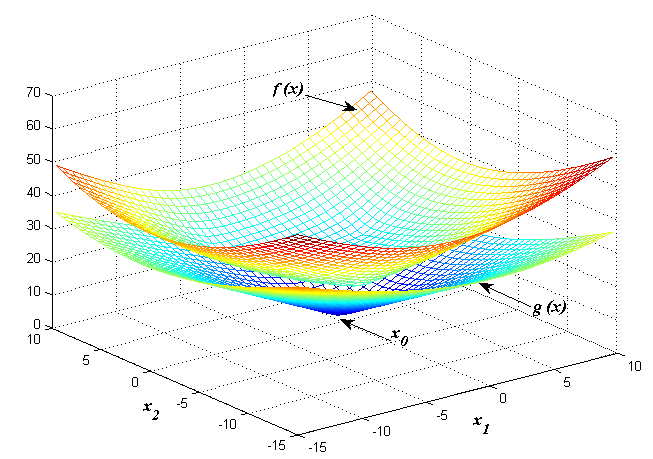
\includegraphics[height=0.7\textheight]{../figures/ccp/ccp_b.png}
\caption{Separation of the nonconvex function into two convex functions.}
\label{fig:ccp_b}
\end{figure}
\end{frame}

\begin{frame} % Slide 32
\frametitle{An example of the basic CCP procedure}
\begin{figure}[h]
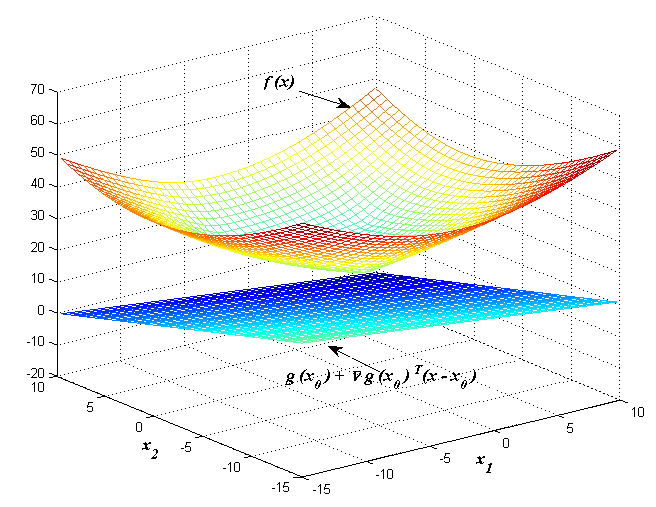
\includegraphics[height=0.7\textheight]{../figures/ccp/ccp_c.png}
\caption{First order approximation of $g(\protect\Bx)$.}
\label{fig:ccp_c}
\end{figure}
\end{frame}

\begin{frame} % Slide 33
\frametitle{An example of the basic CCP procedure}
\begin{figure}[h]
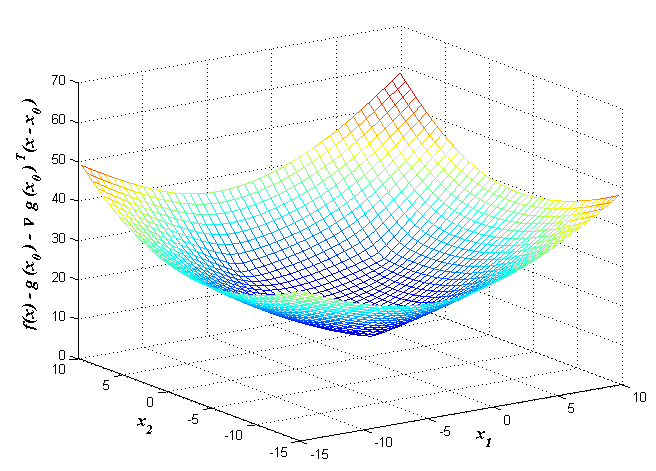
\includegraphics[height=0.7\textheight]{../figures/ccp/ccp_d.png}
\caption{A convex approximation of the original nonconvex function at $\protect\Bx_0 = (0,0)$.}
\label{fig:ccp_d}
\end{figure}
\end{frame}

\begin{frame} % Slide 34
\frametitle{Range-Based Localization Revisited}
\phantom{m}

\phantom{m}

\phantom{m}

\phantom{m}

\begin{itemize}
\item
The range-based least squares (R-LS) estimate:
\nonumber
\begin{equation} \tag{R}
\Min_{\Bx} F(\Bx) = \sum_{i=1}^m \left(r_i  - \|\Bx - \Ba_i\| \right)^2
\end{equation}
\end{itemize}
\end{frame}


\begin{frame} % Slide 35
\frametitle{Problem Reformulation} 
\phantom{m}
\begin{itemize}
\item
We begin by re-writing the objective $F(\Bx)$ up to a constant as:
\begin{equation}
\nonumber
\begin{aligned} 
 \sum_{i=1}^{m} (r_i - \|{\Bx} - {\Ba}_i\|)^2 = m\Bx^T\Bx - 2 \Bx^T\sum^m_{i=1} \Ba_i - 2\sum^m_{i = 1} r_i \|\Bx - \Ba_i\|
\end{aligned}
\end{equation}
which allows to formulate it in a basic CCP form $F(\Bx) = f(\Bx) –- g(\Bx)$ \\
with 
\begin{equation}
\nonumber
\begin{aligned}
& f(\Bx)  =  m \Bx^T\Bx - 2 \Bx^T\sum^m_{i=1} \Ba_i & {} & \mbox{ - convex} \\
& g(\Bx) =  2 \sum^m_{i = 1} r_i \|\Bx - \Ba_i\| & {} & \mbox{ - convex} .
\end{aligned}
\end{equation}

\end{itemize}
\end{frame}

\begin{frame} % Slide 36 
\frametitle{Problem Reformulation} 
\phantom{m}
\begin{itemize}
\item
Since  $g(\Bx)$ is not differentiable at the point where $\Bx = \Ba_i$ for some $1 \leq i \leq m$,  we replace  $\bigtriangledown g(\Bx_k)$ by a subgradient of $g(\Bx)$ at  $\Bx_k$  as
\begin{equation} 
\nonumber
\partial g{(\Bx_k)}  = 2 \sum^m_{i = 1} r_i \partial \|\Bx_k - \Ba_i\| 
\end{equation}
\mbox{where }
\begin{equation}
\nonumber
\partial \|\Bx_k - \Ba_i\|  = \left\{
	\begin{aligned}
	& \frac{\Bx_k - \Ba_i}{\|\Bx_k - \Ba_i\|}, &\mbox{if } \Bx_k \neq \Ba_i \\
	& \BO, &\mbox{otherwise }
	\end{aligned}
\right.
\end{equation}
 
\end{itemize}
\end{frame}

\begin{frame} % Slide 37
\frametitle{Problem Reformulation} 
\phantom{m}
\begin{itemize}
\item
Up to a multiplicative factor $1/m$ and an additive constant term the objective in (R) can  be written as 
%Up to a multiplicative factor $1/m$ and a constant  the convex objective function in (R) can  be written as 
\begin{equation}
\nonumber
\Min_{\Bx} \quad \hat{F}(\Bx) = \Bx^T\Bx - 2\Bx^T \Bv_k
\end{equation}
where
\begin{equation}
\begin{aligned}
\nonumber
\Bv_k  = \bar{\Ba} + \frac{1}{m} \sum^m_{i=1} r_i \partial \|\Bx_k - \Ba_i\| , \quad \bar{\Ba} = \frac{1}{m}  \sum^m_{i = 1} \Ba_i 
\end{aligned}
\end{equation}

\item
Given $\Bx_k$ (in the $k$-th iteration) the solution of the quadratic problem can be obtained as
\begin{equation} 
\nonumber
\Bx_{k+1} = \bar{\Ba} + \frac{1}{m} \sum^m_{i=1} r_i \partial \|\Bx_k - \Ba_i\|
\end{equation}
\end{itemize}
\end{frame}



\begin{frame} % Slide 38
\frametitle{Imposing Error Bounds} 
\phantom{m}
\begin{itemize}
\item
The algorithm can be enhanced by imposing a bound on each squared measurement error
\begin{equation} 
\nonumber
\left(\|\Bx - \Ba_i\| - r_i \right)^2 \leq \delta_i^2
\end{equation}
which leads to
\begin{eqnarray} 
\nonumber
\begin{aligned}
\|\Bx - \Ba_i\| - r_i -  \delta_i  & \leq  0 &{} & (C1) \\ 
r_i - \delta_i & \leq  \|\Bx - \Ba_i\|,   & \mbox{for } 1 \leq i \leq m. \quad & (C2)
\end{aligned}
\end{eqnarray} 
 Both sets of constraints can be written in a form $f_i(\Bx) \leq g_i(\Bx) $.   \\~\\

\item
Constraints in  (C1) are convex, with $f_i(\Bx)  = \|\Bx - \Ba_i\|  -  r_i  -  \delta_i$, and $g_i(\Bx)  =  0$. \end{itemize}
\end{frame}

\begin{frame} % Slide 39
\frametitle{Imposing Error Bounds} 
\begin{itemize}
\item
In case of (C2): define $f_i(\Bx) =r_i - \delta_i  $ and $g_i(\Bx) =  \|\Bx - \Ba_i\|$.  \\
Replace $g_i(\Bx)$ with its approximation
% Following CCP, $g_i(\Bx)$ is  linearized around iterate $\Bx_k$ to 
\begin{equation}
\nonumber
\hat{g_i}(\Bx,\Bx_k) = \| \Bx_k - \Ba_i\| + \partial \|\Bx_k - \Ba_i \| ^T \left( \Bx - \Bx_k \right)
\end{equation}
This allows to convexify constraints $r_i - \delta_i  \leq  \|\Bx - \Ba_i\|$ as
\begin{equation}
\nonumber
- \|\Bx_k - \Ba_i \| - \partial \|\Bx_k - \Ba_i \| ^T \left( \Bx - \Bx_k\right) + r_i - \delta_i \leq 0 
\end{equation}

\item
Summarizing, the problem in the $k$-th iteration can be stated as
\setlength{\belowdisplayskip}{0pt} \setlength{\belowdisplayshortskip}{0pt}
\begin{eqnarray}
\nonumber
  \Min_{\Bx}&&\Bx^T\Bx - 2\Bx^T \Bv_k \\
\nonumber
\ \ \qquad \mbox{subject to:}&&\| \Bx - \Ba_i\| - r_i - \delta_i \leq 0 
\end{eqnarray}
\begin{eqnarray}
\nonumber
  -\|\Bx_k-\Ba_i\|-\partial\|\Bx_k-\Ba_i\|^T\left(\Bx-\Bx_k\right) +r_i-\delta_i\leq 0 \quad
\end{eqnarray}
\end{itemize}
\end{frame}

\begin{frame} % Slide 40
\frametitle{ Penalty CCP (PCCP) } 
\begin{itemize}
\item
Technical problem: the formulation requires a feasible initial point $\Bx_0$. \\~\\

\item
Solution approach: allow \textit{infeasible} initinial points by introducing slack variables {$s_i \geq 0, \hat{s_i} \geq 0$, $ 1\leq i \leq m$} into constraints (C1) and (C2) and penalizing the sum of violations. 
 \\~\\
\item
This leads to a \textit{penalty} CCP:% based formulation: 
\setlength{\belowdisplayskip}{0pt} \setlength{\belowdisplayshortskip}{0pt}
\begin{eqnarray} % eq:16
\nonumber
  \Min_{\Bx, \Bs, \hat{\Bs}}&&\Bx^T\Bx - 2\Bx^T \Bv_k + \tau_k \sum^m_{i=1} (s_i + \hat{s_i}) \qquad \  \\
\nonumber
\mbox{subject to:}&&\| \Bx - \Ba_i\| - r_i - \delta_i \leq s_i  
\end{eqnarray}
\begin{eqnarray}
\nonumber
 -\| \Bx_k - \Ba_i\| -\frac{(\Bx_k - \Ba_i)^T}{\| \Bx_k - \Ba_i\|}\left(\Bx - \Bx_k\right) + r_i - \delta_i   \leq \hat{s_i} \\
\nonumber
\qquad s_i \geq 0,  \hat{s_i}  \geq 0, \ \mbox{for: }  i = 1, 2, \ldots, m  
\end{eqnarray}
where $ 0 \leq \tau_k \leq \tau_{max}$.
\\~\\
\end{itemize}
\end{frame}


\begin{frame} % Slide 41
\frametitle{The Algorithm: Input parameters}
{\large \textit{Bound $\delta_i$ on the measurement error}}
\\~\\
\begin{itemize}
\item
Lower $\delta_i$ leads to a ``tighter'' solution.
\\~\\
\item
 Larger $\delta_i$ makes the algorithm less sensitive to outliers.
\\~\\
\item
 If $\Beps$ obeys a Gaussian distribution with zero mean and $\symb{\Sigma} = \mbox{diag}(\sigma_1^2, \ldots, \sigma_m^2)$, then $\delta_i = \gamma \sigma_i$, where $\gamma$ determines the width of  confidence interval.
 \\~\\
 \item
 For example, for $\gamma = 3$ we have the probability $Pr\{|\varepsilon_i| \leq 3\sigma_i\} \approx 0.99$.

\end{itemize}
\end{frame}

\begin{frame} % Slide 42 
\frametitle{The Algorithm: Input parameters}
{\large \textit{Initial point $\Bx_0$}}
\\~\\
Techniques to select a good initial point:
\begin{itemize}
\item
select the initial point uniformly randomly over the same region as the unknown source; 
\\~\\
\item
set the initial point to the origin; \\~\\
\item
run the algorithm from a set of candidate initial points and identify the solution as the one with lowest LS error; %Typically, comparing the results from $n$ distinct initial points shall suffice; %For the planar case ($n = 2$), for example, it is sufficient to compare the two intersection points of the two circles that are associated with the two smallest distance readings as the target is very likely to be in the vicinity of these sensors; 
\\~\\
\item
apply a \textit{global} localization algorithm  to generate an approximate LS solution, then take it as the initial point.% to run the proposed algorithm. 
\end{itemize}
\end{frame}


\subsection{Numerical Results}

\begin{frame} % Slide 43
\frametitle{Numerical Results}
{\large \textit{System setup}}
\\~\\
\begin{itemize}
\item
Sensors: $\{\Ba_i, i = 1, 2,\ldots,5\}$ randomly placed in the planar region in $[-15;15]\times[-15;15]$
\\~\\
\item
Source: $\Bx_s$, located randomly in  $\{\Bx=[x_1;x_2], -10\leq x_1,x_2\leq 10\}$
\\~\\
\item
Noise: $\{\varepsilon_i, i=1,\ldots,m\}$ was modelled as i.i.d random variables with zero mean and variance $\sigma^2$,  $\sigma \in \{10^{-3}, 10^{-2}, 10^{-1}, 1\}$
\\~\\
\item
$\gamma  = 3$, $K_{max} = 20$
\end{itemize}
\end{frame}



\begin{frame} % Slide 44
\frametitle{Numerical Results}
\begin{table}
\centering
\caption{Averaged MSE for SR-LS and PCCP methods}
\begin{tabular}{||c||c|c|c|c||} 
\hhline{|t:=====:t|} 
&&&& \\
%& & & Relative\\  
\textsc{\textbf{$\sigma$}} & \textsc{MLE} & \textsc{SR - LS}& \textsc{PCCP} &\textsc{R.I.} \\%elative improvement}\\ % \hhline
%&&&& \\ 
\hhline{|:=====:|}
&&&& \\ 
{\fontsize{9}{10}\selectfont 1e-03}& {\fontsize{9}{10}\selectfont 6.0159e-01} & {\fontsize{9}{10}\selectfont1.3394e-06}   &	\textbf{{\fontsize{9}{10}\selectfont 9.5243e-07}}& {\fontsize{9}{10}\selectfont 29\%}	 \\ &&&&\\
{\fontsize{9}{10}\selectfont1e-02}& {\fontsize{9}{10}\selectfont 3.5077e-01} & {\fontsize{9}{10}\selectfont1.4516e-04}     &	\textbf{{\fontsize{9}{10}\selectfont9.5831e-05}}& {\fontsize{9}{10}\selectfont34\%}	\\ &&&&\\
{\fontsize{9}{10}\selectfont1e-01}& {\fontsize{9}{10}\selectfont3.7866e-01} & {\fontsize{9}{10}\selectfont1.2058e-02}     &	\textbf{{\fontsize{9}{10}\selectfont8.7107e-03}}& {\fontsize{9}{10}\selectfont28\%}	\\ &&&&\\
{\fontsize{9}{10}\selectfont1e+0}& {\fontsize{9}{10}\selectfont1.4470e+00} & {\fontsize{9}{10}\selectfont1.3662e+00}      &	\textbf{{\fontsize{9}{10}\selectfont1.2346e+00}}& {\fontsize{9}{10}\selectfont10\%}	\\ &&&&\\
\hhline{|b:=====:b|} 
\end{tabular}
\label{tab:1}
\end{table}
\end{frame}

\begin{frame} % Slide
\frametitle{}
\phantom{m}
\begin{itemize}
\item

\end{itemize}
\end{frame}

%------------------------------------------------
%------------------------------------------------
\subsection{Conclusion} 

\begin{frame}
\frametitle{Conclusion} 
\phantom{m}
\begin{itemize}
\item
New iterative method for locating a radiating source based on noisy range measurements
\\~\\
\item
Transforms original least-squares problem to a DC programming problem
\\~\\
\item
This in turn is relaxed to a sequential convex minimization based on PCCP that can be efficiently solved with an infeasible initial point
\\~\\
\item
CCP allows a natural embedding of the LS formulation for localization into a sequential convex formulation
\end{itemize}
\end{frame}

%------------------------------------------------

\begin{frame} [noframenumbering]
\frametitle{  }
\phantom{m} 
\phantom{m}
\phantom{m} 
\phantom{m}
\phantom{m} 
\phantom{m}
\Huge{\centerline{Q \& A }}

\end{frame}

%%------------------------------------------------
%
\appendix
\begin{frame} [noframenumbering]
\frametitle{  }
\phantom{m} 
\phantom{m}
\phantom{m} 
\phantom{m}
\phantom{m} 
\phantom{m}
\Huge{\centerline{Appendix}}
\end{frame}

%%------------------------------------------------
% A.1
\begin{frame}
\frametitle{Nonconvexity of the objective}
\phantom{m}
\linespread{0.1} \selectfont
Given the objective
\begin{equation}
 F(\Bx)= \sum_{i=1}^{m} (r_i - \|{\Bx} - {\Ba}_i\|)^2 \nonumber
\end{equation}
\linespread{1}\selectfont
its Hessian for points $\Bx$ that are not coincided with $\Ba_i$ for $1 \leq i \leq m$, is given by
\begin{equation}
\begin{aligned}
\nonumber
\bigtriangledown ^2 F(\Bx)  = 2m\BI  + &2\sum^m_{i=1} \frac{r_i}{\|\Bx - \Ba_i\|^3} \cdot \\
\cdot &\left( \left(\Bx - \Ba_i\right)\left(\Bx - \Ba_i\right)^T - \|\Bx - \Ba_i\|^2 \BI \right)
\end{aligned}
\end{equation}
which is not always positive semidefinite. Hence $F(\Bx)$ is not convex.
\end{frame}

%%------------------------------------------------
% A.2
\begin{frame} 
\frametitle{Problem Reformulation}
We express the objective in (R) as $F(\Bx) = f(\Bx) –- g(\Bx)$ with 
 \begin{equation}  \nonumber 
f(\Bx) =  
m \Bx^T\Bx - 2 \Bx^T\sum^m_{i=1} \Ba_i \ \ \mbox{and } \ g(\Bx) = 2 \sum^m_{i = 1} r_i \|\Bx - \Ba_i\| 
\end{equation}
  
Then, we replace $\bigtriangledown g(\Bx_k)$ by a subgradient of $g(\Bx)$ at $\Bx_k$:
\begin{equation} 
\nonumber
\partial g{(\Bx_k)}  = 2 \sum^m_{i = 1} r_i \partial \|\Bx_k - \Ba_i\|, 
\end{equation}
where 
\begin{equation}
\nonumber
\partial \|\Bx_k - \Ba_i\|  = \left\{
	\begin{aligned}
	& \frac{\Bx_k - \Ba_i}{\|\Bx_k - \Ba_i\|}, &\mbox{if } \Bx_k \neq \Ba_i \\
	& \BO, &\mbox{otherwise }
	\end{aligned}
\right.
\end{equation}
\end{frame}

\begin{frame} 
\frametitle{Problem Reformulation}
\phantom{m}
Hence  $ \hat{g}(\Bx,\Bx_k) $ can be formed as: 
\begin{equation} 
\nonumber
\begin{aligned}
  \hat{g}(\Bx,\Bx_k)   & =   g(\Bx_k) +  \bigtriangledown g(\Bx_k)^T(\Bx - \Bx_k) \\
  & =   2 \sum^m_{i=1} r_i \|\Bx_k - \Ba_i\|   +  2 \left( \Bx - \Bx_k \right)^{T} \sum^m_{i=1} r_i \partial \|\Bx_k - \Ba_i\| \\
& = 2\Bx^T \sum^m_{i=1} r_i \partial \|\Bx_k - \Ba_i \| + c
\end{aligned}
\end{equation} 
where $c$ is a constant given  by
\begin{equation} 
\nonumber
 c = - 2 \sum_{i = 1}^m r_i \Ba_i^T \partial \|\Bx_k - \Ba_i\|.
\end{equation} 
\end{frame}

%%------------------------------------------------
% A.3
\begin{frame}
\frametitle{The Algorithm}
%\phantom{m}
{\large \textit{PCCP-based LS Algorithm for Source Localization}}
\\~\\
\textbf{Step 1:} Input sensor locations $\{\Ba_i, i = 1,\ldots,m\}$, range measurements $\{r_i, i = 1, \ldots, m\}$, $\Bx_0, K_{max}, \tau_0, \tau_{max}, \mu > 0, \gamma, \sigma$, and set $k = 0$. 
\\~\\
\textbf{Step 2:} Form  $\Bv_k$ and solve PCCP. Denote the solution as  $(\Bs^*, \hat{\Bs}^*, \Bx^*)$. 
\\~\\
\textbf{Step 3:} Update  $\tau_{k+1} $ = min $(\mu\tau_k, \tau_{max})$, set $k = k+1$. 
\\~\\
\textbf{Step 4:} If $k = K_{max}$, terminate and output $\Bx^*$ as the solution; otherwise, set $\Bx_k = \Bx^*$ and repeat from Step 2. 
\end{frame}

%%%%%%%%%%%%%
%%%b IRW
%%%%%%%%%%%%%
\section{Conclusions}

\begin{frame}
\frametitle{Conclusions}
\phantom{m}
\phantom{m}
\begin{itemize}
\item <2->
New global methods for locating a radiating source based on noisy range or range difference measurements have been proposed. \\~\\
\item <3->
These methods are developed by transforming the SR-LS and SRD-LS algorithms [BSL2008] into an iterative procedure % where adaptively weighted SR-LS (SRD-LS) objective is minimized so as to move a weighted SR-LS (SRD-LS) objective towards the original R-LS objective as the iteration continues. \\~\\
so that a weighted SR-LS (SRD-LS) objective asymptotically approaches the original R-LS objective. \\~\\
\item <4->
Proposed algorithms are found to outperform the existing methods.
\end{itemize}
\end{frame}

%------------------------------------------------

\begin{frame} [noframenumbering]
\frametitle{  }
\phantom{m} 
\phantom{m}
\phantom{m} 
\phantom{m}
\phantom{m} 
\phantom{m}
\Huge{\centerline{Q \& A }}

\end{frame}

%%------------------------------------------------
%
\appendix
\begin{frame} [noframenumbering]
\frametitle{  }
\phantom{m} 
\phantom{m}
\phantom{m} 
\phantom{m}
\phantom{m} 
\phantom{m}
\Huge{\centerline{Appendix}}
\end{frame}

% A.1
\begin{frame}
\frametitle{Source Localization From Range Measurements}
{\large \textit{Weighted Squared Range Least Squares Formulation}} \\
\normalsize
\begin{itemize}
\item
Following [BSL2008], we convert \eqref{WSR} into a GTRS as
\begin{eqnarray} \label{1} %eq 6 a,b
\setcounter{abc}{1}
\Min_{{\By} \in R^{n+1}} \|\BA_w\By-\Bb_w\|^2 \qquad\\
\stepcounter{abc} \setcounter{equation}{1} \mbox{subject to: \ }
\By^T\BD\By + 2\Bf^T\By = 0
\end{eqnarray}
where $\By = [\Bx^T \ \alpha]^T$, $\alpha = \|\Bx\|$, $\BA_w = \BGA\BA$ and $\Bb_w = \BGA\Bb$ with fixed $\BGA=\mbox{diag}\left(\sqrt{w_1},\ldots,\sqrt{w_m}\right)$, and

\begin{equation} \label{2}
\setcounter{equation}{2}
\setcounter{abc}{0}
\BA=\left(\begin{array}{cc}
    -2\Ba_1^T & 1 \\
    \vdots  & \vdots \\
    -2\Ba_m^T & 1
    \end{array} \right),
\Bb=\left(\begin{array}{c}
    r_1^T-\|\Ba_1\|^T \\
    \vdots \\
    r_m^T-\|\Ba_m\|^T
    \end{array} \right)
\end{equation}
\begin{equation} \label{3}
\BD=\left(\begin{array}{cc}
    \BI\!_{n\times n} & \BO_{n\times 1} \\
    \BO_{1\times n} & 0
    \end{array} \right),
\Bf=\left(\begin{array}{c}\BO \\ -0.5 \end{array} \right)
\end{equation}
%For a \textit{fixed} set of weights $\{w_i, i = 1, …, m\}$, the global solution of (6) can be solved by the method developed in and we denote the solution by  $\mathbf{S}(\BA_w, \Bb_w, \BD, \Bf)$.
\end{itemize}
\end{frame}

%%------------------------------------------------
%\begin{frame}
%\frametitle{Source Localization From Range Measurements}
%{\large \textit{An Iterative Re-Weighting Strategy}} \\
%\normalsize
% More importantly, when the iterates produced by solving (\ref{eq:12}) (namely $\Bx_k$ for $k = 1, 2,\ldots$) converge, in the $k$th iteration with $k$ sufficiently large, the objective function of (\ref{eq:11}) in a small vicinity of its solution $\Bx_k$ is approximately equal to
%\begin{equation} \label{sr:w}
%\nonumber
%\begin{aligned}
%&\sum_{i=1}^m w_i^{(k)}\left(\|\Bx-\Ba_i\|^2-r_i^2\right)^2 \\ % \approx \sum_{i=1}^m w_i^{(k)}\left(\|\Bx_k-\Ba_i\|^2-r_i^2\right)^2 \\
%%&=\sum_{i=1}^m w_i^{(k)}\left(\|\Bx_k-\Ba_i\|+r_i\right)^2\left(\|\Bx_k-\Ba_i\|-r_i\right)^2  \\
%& \approx \sum_{i=1}^m w_i^{(k)}\left(\|\Bx_{k-1}-\Ba_i\|+r_i\right)^2\left(\|\Bx_k-\Ba_i\|-r_i\right)^2 
%%&=\sum_{i=1}^m \left(\|\Bx_k-\Ba_i\|-r_i\right)^2 
% \approx \sum_{i=1}^m \left(\|\Bx-\Ba_i\|-r_i\right)^2\\
%\\
%\end{aligned}
%\end{equation}
%\end{frame}
%%------------------------------------------------

% A.2
\begin{frame}
%\frametitle{An Iterative Re-Weighting Strategy}
\frametitle{Source Localization From Range Measurements}
{\large \textit{The Algorithm}} \\
\normalsize
% The localization method can be outlined as follows.
\begin{enumerate}
\item %1
\underline{Input data}: Sensor locations $\{\Ba_i, i=1,\ldots,m\}$, range measurements $\{r_i, i=1,\ldots,m\}$, maximum number of iterations $k_{max}$ and convergence tolerance $\zeta$.
\item %2
Generate data set $\BA,\Bb, \BD, \Bf$ using (2) and \eqref{3}. Set $k=1, w_i^{(1)}=1$ for $i=1,\ldots,m$.
\item %3 
Set $\BGA_k=\mbox{diag}\left(\sqrt{w_1^{(k)}},\ldots,\sqrt{w_m^{(k)}}\right)$, $\BA_w=\BGA_k\BA$ and $\Bb_w=\BGA_k\Bb$.
\item%4
Solve the WSR-LS problem \eqref{IRWSR}  via (1) to obtain its global solution $\Bx_k$. % = $ \mathbf{S}(\BA_w, \Bb_w, \BD, \Bf)$.
\item %5
If $k=k_{max}$ or $\|\Bx_k-\Bx_{k-1}\|<\zeta$, terminate and \underline{output $\Bx_k$} as the solution; otherwise, set $k=k+1$, update weights $\{w_i^{(k)}, i=1,\ldots,m\}$ and repeat from Step 3).
\end{enumerate}
\end{frame}
%%------------------------------------------------

%\begin{frame}
%\frametitle{The Algorithm}
%It is evident that the complexity of the algorithm is practically equal to the complexity of the WSR-LS solver involved in Step 4 times the number of iterations, $k$. The algorithm converges with a small number of iterations, typically a $k \leq 6$ suffices. Convergence is guaranteed due to the nature of the WSR-LS solver which produces a global solution that does not depend on the initial point, and convexity of the WSR-LS problem (6). For simplicity, we shall call the solutions obtained from Algorithm 1 IRWSR-LS solutions.
%\end{frame}

%------------------------------------------------

% A.3
\begin{frame}
\frametitle{Source Localization From Range-Difference Measurements} %3.2
{\large \textit{Weighted Squared Range-Difference Least Squares Formulation}} \\~\\
\normalsize
\begin{itemize}
\item 
By introducing new variable $\By=[\Bx^T \ \|\Bx\|]^T$ and noticing nonnegativity of the component $y_{n+1}$ problem \eqref{WSRD} is converted to
\begin{eqnarray} \label{4}
\setcounter{abc}{0} \stepcounter{abc}
\Min_{\By \in R^{n+1}} \|\BB_w\By - \Bg_w\| \\
\stepcounter{abc} \setcounter{equation}{4}
\mbox{subject to: } \By^T\BC\By = 0 \\
\stepcounter{abc} \setcounter{equation}{4}
y_{n+1}\geq 0
\end{eqnarray}
\item
where $\BB_w=\BGA\BB$, $\Bg_w=\BGA\Bg$ , $\BGA=\mbox{diag}\{\sqrt{w_1},\ldots,\sqrt{w_m}\}$,  $\Bg=[g_1 \ldots g_m]^T$ and
\begin{equation} \label{5}
\setcounter{abc}{0}
%\label{eq:20} %29
\BB = \left(\begin{array}{cc}
    -2\Ba_1^T & -2d_1 \\
    \vdots & \vdots \\
    -2\Ba_m^T & -2d_m
    \end{array}\right),
\BC =  \left(\begin{array}{cc}
    \BI_n & \BO_{n \times 1} \\
    \BO_{1 \times n} & -1
    \end{array}\right)
\end{equation}

%On comparing (23) with (19), it follows immediately that the global solver for problem (19) characterized by data set $\{\BB, \Bg, \BC\}$ can also be used for solving problem (23) by applying it to data set $\{\BB_w, \Bg_w, \BC\}$.

\end{itemize}
\end{frame}
%------------------------------------------------
%\begin{frame}
%\frametitle{SRD-LS Formulation}
%Reference [12] presents a rigorous argument which shows that the optimal solution of (\ref{eq:19}) either assumes the form of  $\tilde{\By}(\lambda)=\left(\BB_w^T\BB_w+\lambda\BC\right)^{-1}\BB^T\Bg$
% where $\lambda$ solves
% \begin{equation}\label{eq:21}
% \tilde{\By}(\lambda)^T\BC\tilde{\By}(\lambda)=0
% \end{equation}
% and makes $\BB^T\BB+\lambda\BC$ positive definite, or is the vector among $\{\BO,$ $\tilde{\By}(\lambda_1),\ldots,\tilde{\By}(\lambda_p)\}$ that gives the smallest objective function in (\ref{eq:19}a), where $\{\lambda_i, i = 1,\ldots,p\}$ are all roots of (\ref{eq:21}) such that the $(n+1)$'th component of $\tilde{\By}(\lambda_i)$ is nonnegative and $\BB^T\BB+\lambda\BC$ has exactly one negative and $n$ positive eigenvalues. We shall refer the global solution of (\ref{eq:19}) to as the SRD-LS solution.
%\end{frame}

%------------------------------------------------
% A.4 
\begin{frame}
%\frametitle{An Iterative Re-Weighting Strategy}
\frametitle{Source Localization From Range Difference Measurements}
{\large \textit{The Algorithm}} \\~\\
\normalsize
% The localization method can be outlined as follows.
\begin{enumerate}
\item %1 
\underline{Input data}: Sensor locations $\{\Ba_i, i=0, 1,\ldots,m\}$ with $\Ba_0=\BO$, range-difference measurements $\{d_i, i = 1,\ldots,m\}$, maximum number of iterations $k_{max}$ and convergence tolerance $\xi$.
\item %2
Generate data set $\{\BB, \Bg, \BC\}$ using (5). Set $k=1$, $w_i^{(1)}=1$ for $i=1,\ldots,m.$
\item %3
Set $\BGA_k=\mbox{diag}\left(\sqrt{w_1^{(k)}},\ldots,\sqrt{w_m^{(k)}}\right)$, $\BB_w=\BGA_k\BB$ and $\Bg_w=\BGA_k\Bg$.
\item %4
Solve WSRD-LS problem \eqref{4} to obtain its global solution $\Bx_k$.
\item %5
If $k=k_{max}$ or $\|\Bx_k-\Bx_{k-1}\|<\xi$, terminate and \underline{output $\Bx_k$} as the solution; otherwise, set $k=k+1$, update weights $\{w_i^{(k)}, i=1,\ldots,m\}$ and repeat from Step 3).
%We shall call the solutions obtained from Algorithm 2 IRWSRD-LS solutions.
\end{enumerate}
\end{frame}

%%%%%%%%%%%%%%%%%%%
%%%% PCCCP
%%%%%%%%%%%%%%%%%%%



%------------------------------------------------

% A.5

\begin{frame} [t,allowframebreaks]
\frametitle{References}

%\printbibliography
%\end{frame}
%

\begin{thebibliography}{99} 

\bibitem{1}
%[SA1987] 
J. O. Smith and J. S. Abel, ``Closed-form least-squares source location
estimation from range-difference measurements,'' {\em IEEE Trans. Acoust.,
Speech Signal Process.}, vol. 12, pp. 1661--1669, Dec. 1987.

\bibitem{2}
%[SR1987] 
H. Schau and A. Robinson, ``Passive source localization employing intersecting spherical surfaces from time-of-arrival differences,'' {\em IEEE Trans. Acoust., Speech Signal Process.}, vol. ASSP--35, pp. 1223--1225, Aug. 1987.

\bibitem{3}
%[YHR1998] 
K. Yao, R. Hudson, C. Reed, D. Chen, and F. Lorenzelli, ``Blind beamforming on a randomly distributed sensor array system,'' {\em IEEE J. Select. Areas Commun.}, vol. 16, pp. 1555-1567, Oct. 1998.

\bibitem{4}
%[Sp2001]  
M. A. Sprito, ``On the accuracy of cellular mobile station location estimation,'' {\em IEEE Trans. Veh. Technol.}, vol. 50, pp. 674-685, May 2001.

\bibitem{5}
%[HBE2002] 
Y. Huang, J. Benesty, G. W. Elko, and R. M. Mersereau, ``Realtime passive source localization: A practical linear correction least-squares approach,'' {\em IEEE Trans. Speech Audio Process.}, vol. 9, no. 8, pp. 943-956, Nov. 2002.

\bibitem{6}
%[CSM2004]
K. W. Cheung, H. C. So, W. K. Ma, and Y. T. Chan, ``Least squares algorithms for time-of-arrival-based mobile location,'' {\em IEEE Trans. Signal Process.}, vol. 52, no. 4, pp. 1121--1228, Apr. 2004.

\bibitem{7}
%[LH2004] 
D. Li and H. Hu, ``Least square solutions of energy based acoustic source localization problems,'' in {\em Proc. ICPPW}, 2004.

\bibitem{8}
%[CMS2004] 
K.W. Cheung, W.K. Ma, and H.C. So, ``Accurate approximation algorithm for TOA-based maximum-likelihood mobile location using semidefinite programming,'' in {\em Proc. ICASSP}, 2004, vol. 2, pp. 145--148.

\bibitem{9}
%[STK2005] 
A. H. Sayed, A. Tarighat, and N. Khajehnouri, ``Network-based wireless location,'' {\em IEEE Signal Process. Mag.}, vol. 22, no. 4, pp. 24--40, July 2005.

\bibitem{10}
%[CHC2006] 
Y. T. Chan, H. Y. C. Hang, and P. C. Ching, ``Exact and approximate maximum likelihood localization algorithms,'' {\em IEEE Trans. Veh. Technol.}, vol. 55, no. 1, pp. 10--16, Jan. 2006.

\bibitem{11}
%[SL2006] 
P. Stoica and J. Li, ``Source localization from range-difference measurements,'' {\em IEEE Signal Process. Mag.}, vol. 23, pp. 63--65,69, Nov. 2006.

\bibitem{12}
%[BSL2008] 
A. Beck, P. Stoica and J. Li,  ``Exact and approximate solutions of source localization problems,'' {\em IEEE Trans. Signal Processing}, vol. 56, no. 5, pp. 1770--1777, May 2008.

\bibitem{13}
%[VB1996] 
L. Vandenberghe and S. Boyd, ``Semidefinite programming,'' {\em SIAM Rev.}, vol. 38, no. 1, pp. 40--95, Mar. 1996.

\bibitem{14}
%[AL2007] 
A. Antoniou and W.-S. Lu, {\em Practical Optimization: Algorithms and Engineering Applications}, Springer, 2007.

\bibitem{15}
%[Mo1993] 
J.J. More, ``Generalizations of the trust region subproblem,'' {\em Optim. Methods Softw.}, vol. 2, pp. 189--209, 1993.

\bibitem{16}
%[FW2004] 
C. Fortin and H. Wolkowicz, ``The trust region subproblem and semidefinite programming,'' {\em Optim. Methods Softw.}, vol. 19, no.1, pp. 41--67, 2004.

\end{thebibliography}


%\begin{frame}
%\frametitle{References}
%\footnotesize{
%\begin{thebibliography}{99} % Beamer does not support BibTeX so references must be inserted manually as below
%\bibitem[Smith, 2012]{p1} John Smith (2012)
%\newblock Title of the publication
%\newblock \emph{Journal Name} 12(3), 45 -- 678.
%\end{thebibliography}
%}
\end{frame}

%%--------------------------------------------------
% EXAMPLES %--------------------------------------------------
%%\frametitle{Blocks of Highlighted Text}
%\begin{block}{Block 1}
%Lorem
%\end{block}
%
%\begin{block}{Block 2}
%Pellentesque sed tellus purus.
%\end{block}
%
%\begin{block}{Block 3}
%Suspendisse tincidunt sagittis gravida.
%\end{block}
%\end{frame}

%------------------------------------------------

%\begin{frame}
%\frametitle{Multiple Columns}
%\begin{columns}[c] % The "c" option specifies centered vertical alignment while the "t" option is used for top vertical alignment
%
%\column{.45\textwidth} % Left column and width
%\textbf{Heading}
%\begin{enumerate}
%\item Statement
%\item Explanation
%\item Example
%\end{enumerate}
%
%\column{.5\textwidth} % Right column and width
%Lorem ipsum dolor sit amet, consectetur adipiscing elit. Integer lectus nisl, ultricies in feugiat rutrum, porttitor sit amet augue. Aliquam ut tortor mauris. Sed volutpat ante purus, quis accumsan dolor.
%
%\end{columns}
%\end{frame}



%----------------------------------------------------------------------------------------

\end{document} 